Z tej technologii korzystaliśmy głównie do wyśrodkowania poszczególnych elementów względem środka innego.

\begin{code}
	\lstinputlisting[linerange={14-18}, firstnumber=1]{../meetspace/app/assets/stylesheets/_variables.css.scss}
\end{code}\\

Fragment kodu powyżej to przykład dobrodziejstw preprocesora Sass. \emph{Mixin} to funkcja, która może być wielokrotnie wykorzystana na wielu selektorach CSS.

\begin{code}
	\lstinputlisting[linerange={38-40, 75-75}, firstnumber=1]{../meetspace/app/assets/stylesheets/welcome.css.scss}
\end{code}\\

\emph{@include flex(left)} rozszerzy klasę \emph{search} o właściwości wymienione w pierwszym fragmencie kodu.

\clearpage

Efekty:
\begin{figure}[h]
	\centering
  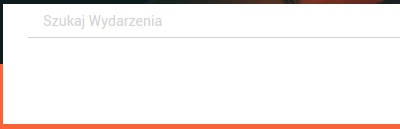
\includegraphics[scale=0.8]{images/flex_before.png}
  \caption{Bez flexbox.}
\end{figure}\\

\begin{figure}[h]
	\centering
  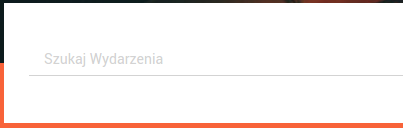
\includegraphics[scale=0.8]{images/flex_after.png}
  \caption{Z wykorzystaniem flexbox.}
\end{figure}

